\chapter{Design}

This chapter details the platform's architecture. It begins with an overview of the architecture and a concise description of its key components. It then provides examples of how these components are deployed and interact with each other, which are covered in detail and displayed with diagrams. The following sections will go deeper into each component.

\section{System Architecture}

\subsection{High-level system architecture}

The platform consists of five main parts: the front end, back end, database, LLM-API, and the AI model, as the figure \ref{fig:high-level-architecture} shows. Each is containerized and can be deployed independently to scale as needed.

\begin{figure}[!h]
    \centering
    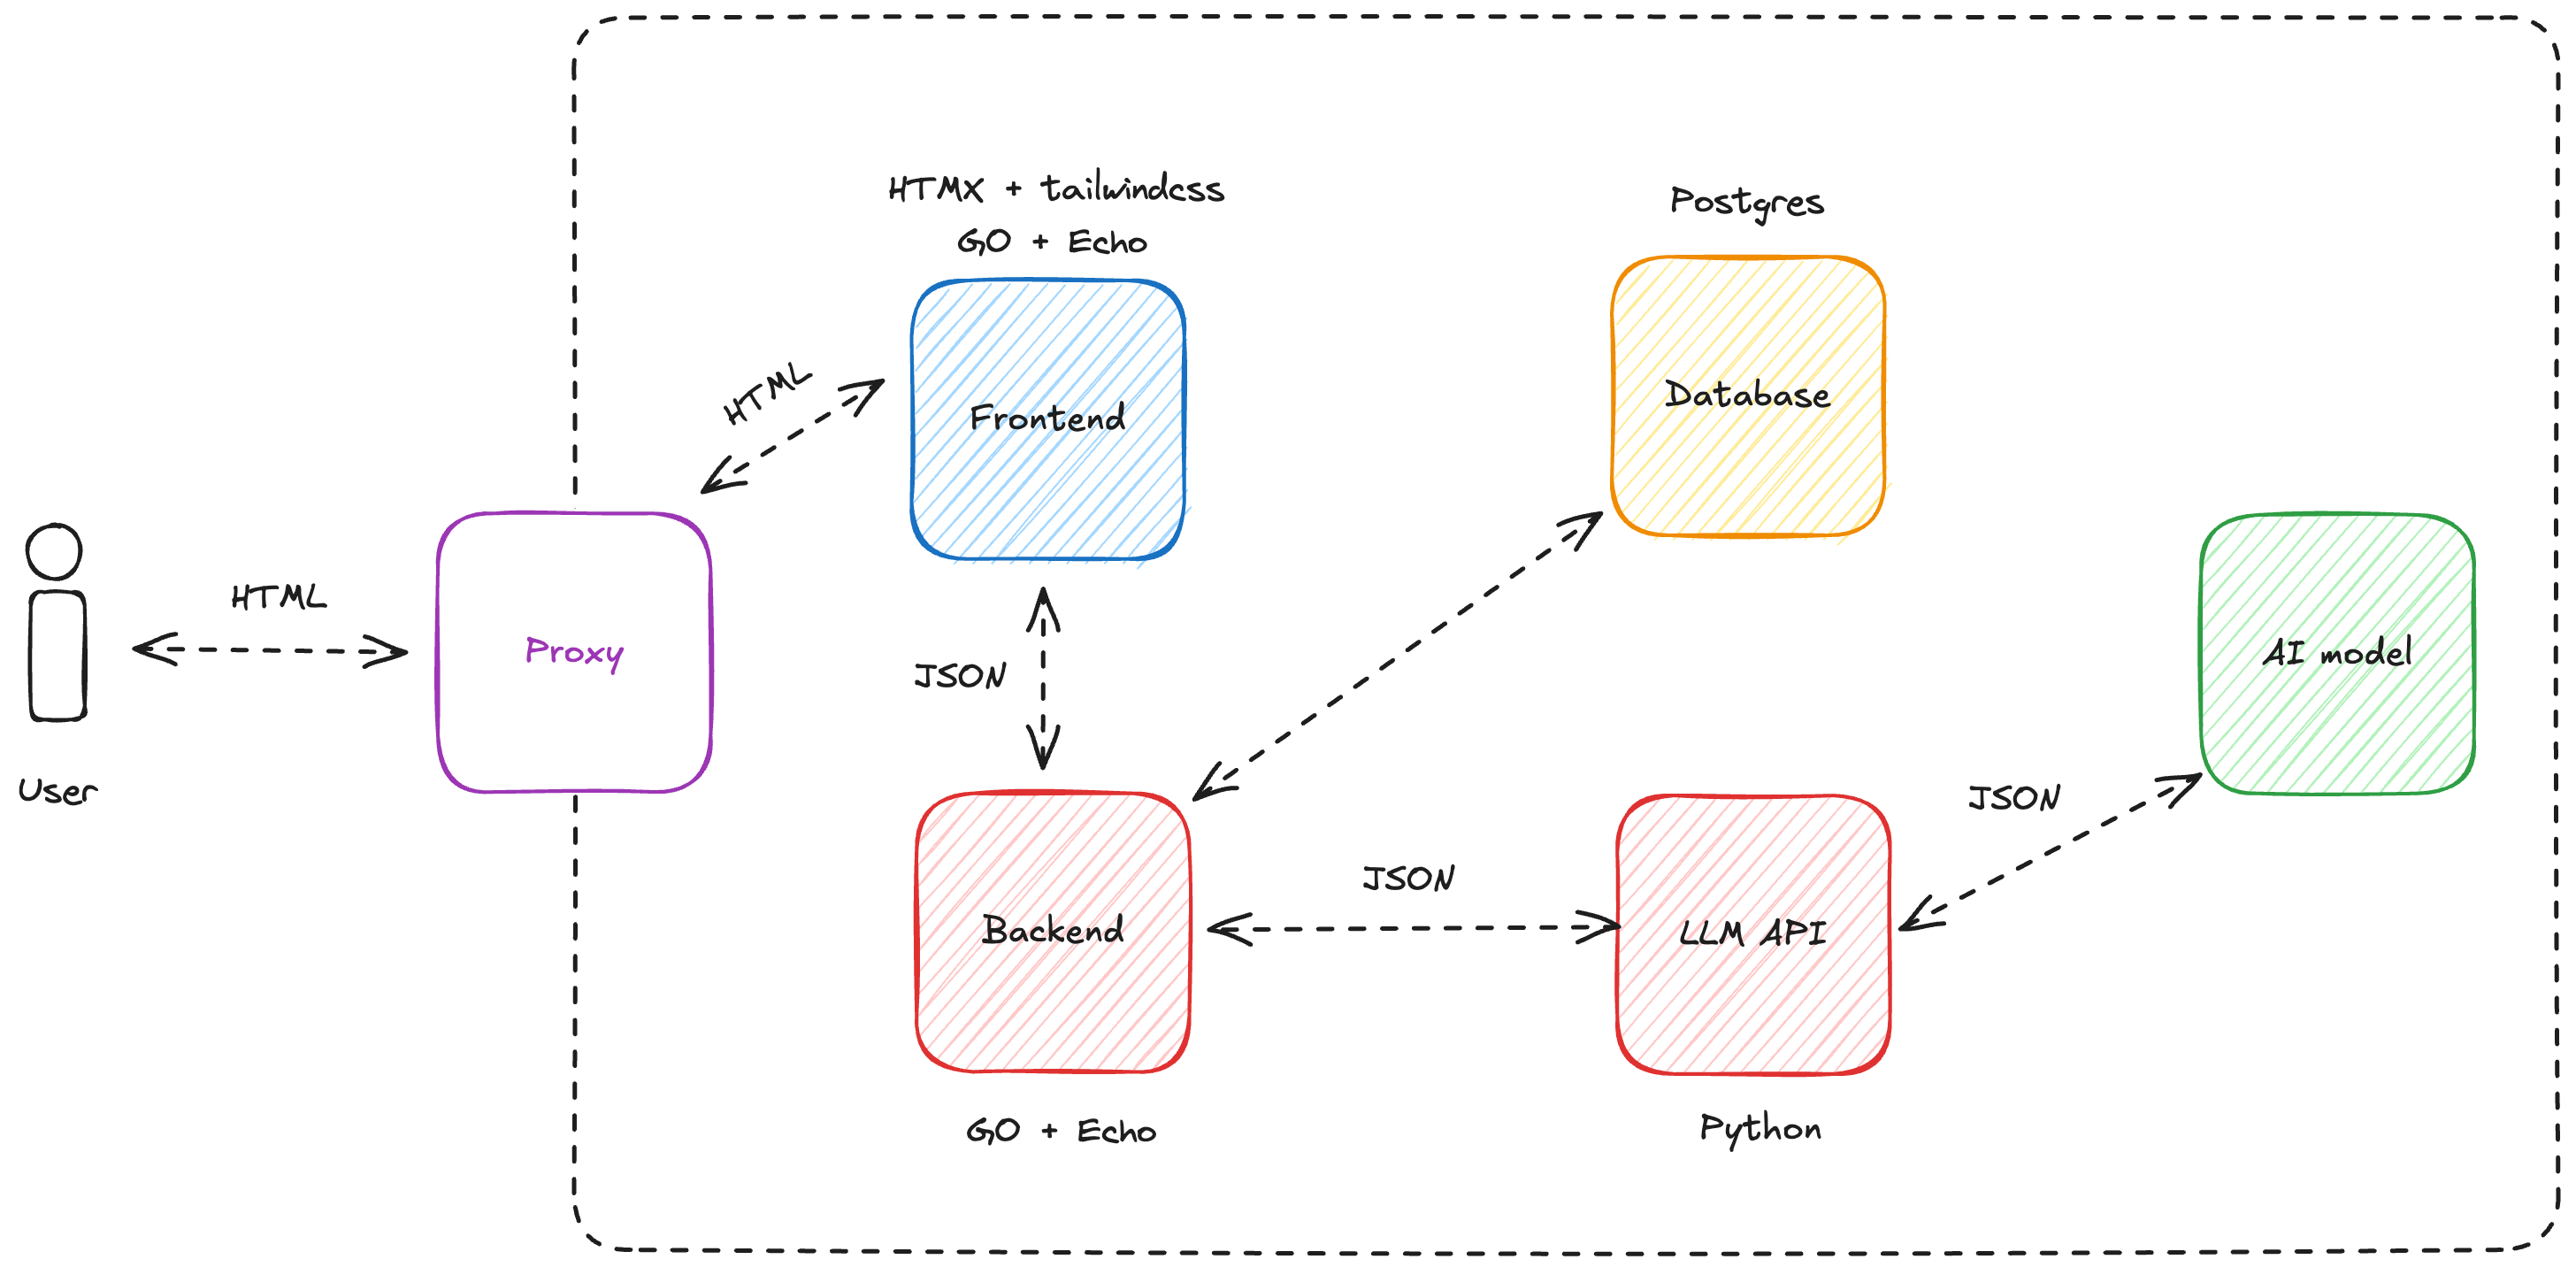
\includegraphics[width=0.8\textwidth, keepaspectratio]{figures/high-level-architecture.png}
    \caption{High-level system architecture}
    \label{fig:high-level-architecture}
\end{figure}

The frontend server is the part of the platform that users interact with directly. It's built as a server-rendered HTMX application using the Go programming language and the Echo framework. As the main entry point to the platform, it processes user inputs, communicates with the backend service, and provides content to users.

The backend is also written in Golang using the Echo framework. It is a regular REST application that communicates with HTTP requests. It brings together the different parts of the application and is responsible for the platform's business logic.

The database is Postgres, a popular, open-source relational database software. It stores all the data so the platform can work seamlessly. This component only communicates with the backend service.

The LLM API component is a unified interface for accessing the AI model. It is a small Python web application with a REST interface for more accessible communication. It contains prompts and question generation-related business logic. The component enables the platform to integrate different AI models or change between them on the fly.

The AI model component is a small application containing the question generator LLM. Máté Debreczeni fine-tuned the pre-trained llama-3-8B\footnote{https://huggingface.co/meta-llama/Meta-Llama-3-8B} model for the platform on a custom dataset he created from Wikipédia articles \footnote{https://en.wikipedia.org/wiki/Wikipedia:Vital_articles}. He aims to train a model that generates better-quality questions in the given format than the starter model.  

\subsection{Example component interaction}

Figure \ref{fig:component-interaction} shows an example interaction between the components through a question generation. This interaction is the primary interaction between the components and utilizes all of them.

\begin{figure}[!h]
    \centering
    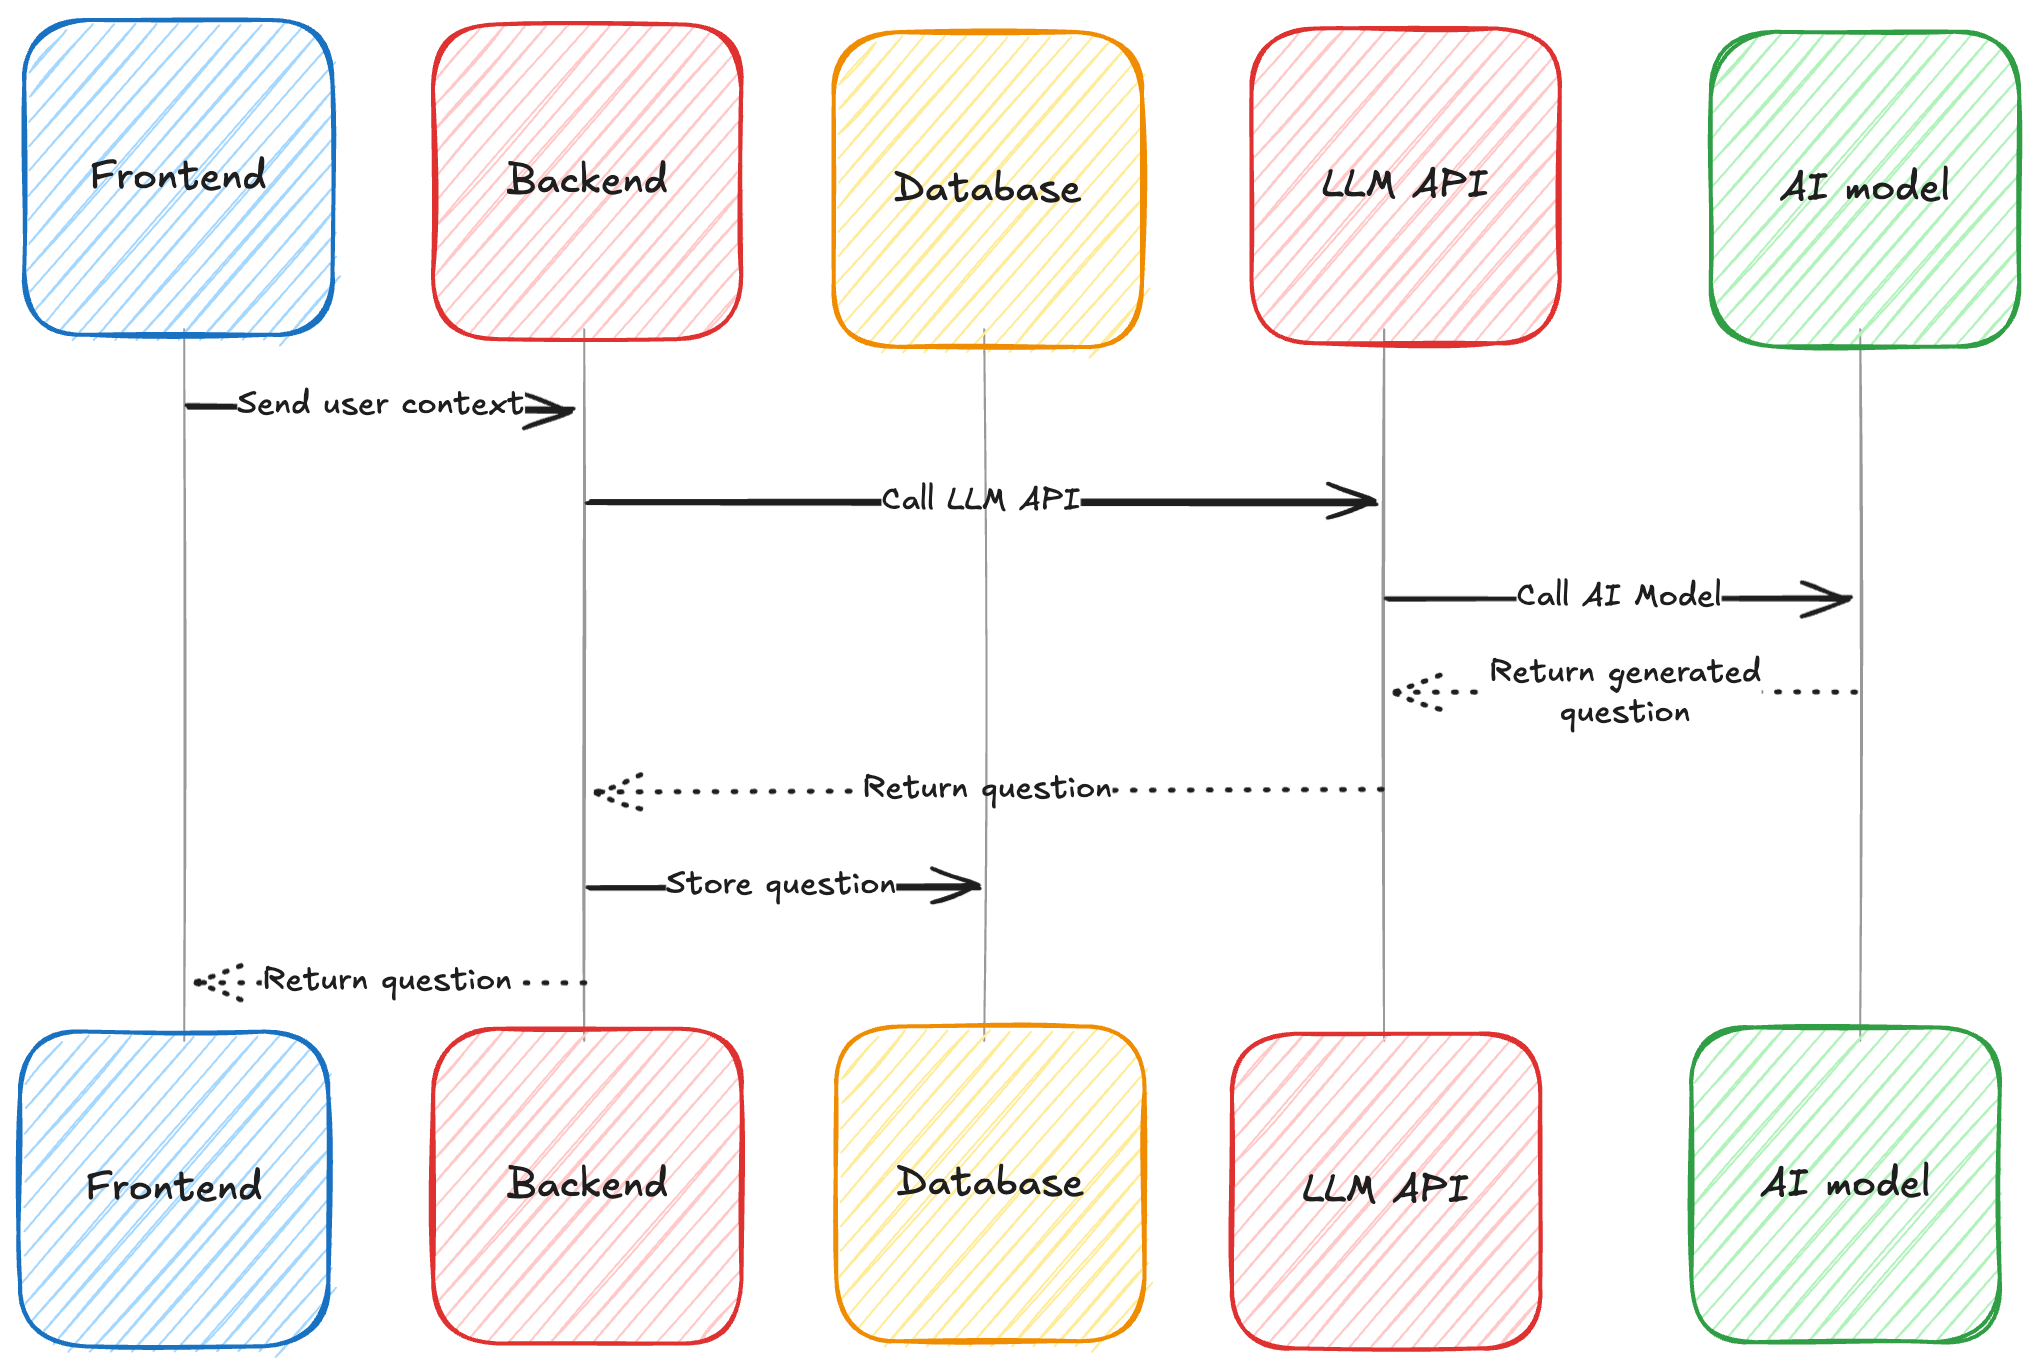
\includegraphics[width=0.8\textwidth, keepaspectratio]{figures/component-interaction.png}
    \caption{Component interaction: Question generation}
    \label{fig:component-interaction}
\end{figure}

Users submit their context to the frontend server, which validates the input and sets parameters like question type and quiz ID. The frontend calls the backend's proper endpoint with these parameters. The backend also validates the request and calls the LLM API to generate the question. The LLM API delegates the generation to the AI model through a request containing a pre-created prompt. This question is returned to the backend, where additional data is added and saved to the database. Finally, the backend returns the question to the frontend for display to the user.

\subsection{Deployment design}

Containerization is a crucial part of platform development and deployment. From the start, all the components were containerized with Docker for easier development and to ensure they worked on other machines. Máté worked on the AI model and the LLM API, and I worked on the other parts. Both of us used different operating systems, software, and tools. Without this method, we could not have worked together as efficiently as we did.

We created a Dockerfile for each service that describes how to build and run the respective application. We configured a docker-compose file to make them work together. We also considered building containers efficiently using the multi-layered containerizing approach. This idea was essential for the frontend and the backend due to the code generation, which has to be performed frequently.

\subsubsection{Development deployment}

Figure \ref{fig:dev-deployment} shows how we deployed locally the platform for development. It consists of two groups: the local environment and the external environment. The local environment has all of the components in the system architecture diagram; this is a complete system. In comparison, the external environment consists of only one service, an LLM from Google. It is the company's fastest Gemini model (gemini-1.5-flash). 

The LLMs, even these smaller ones, need a lot of resources. Thus, question generation usually takes over a minute on a personal computer. We sped up the development process using Gemini's API when developing and testing the services.

\begin{figure}[!h]
    \centering
    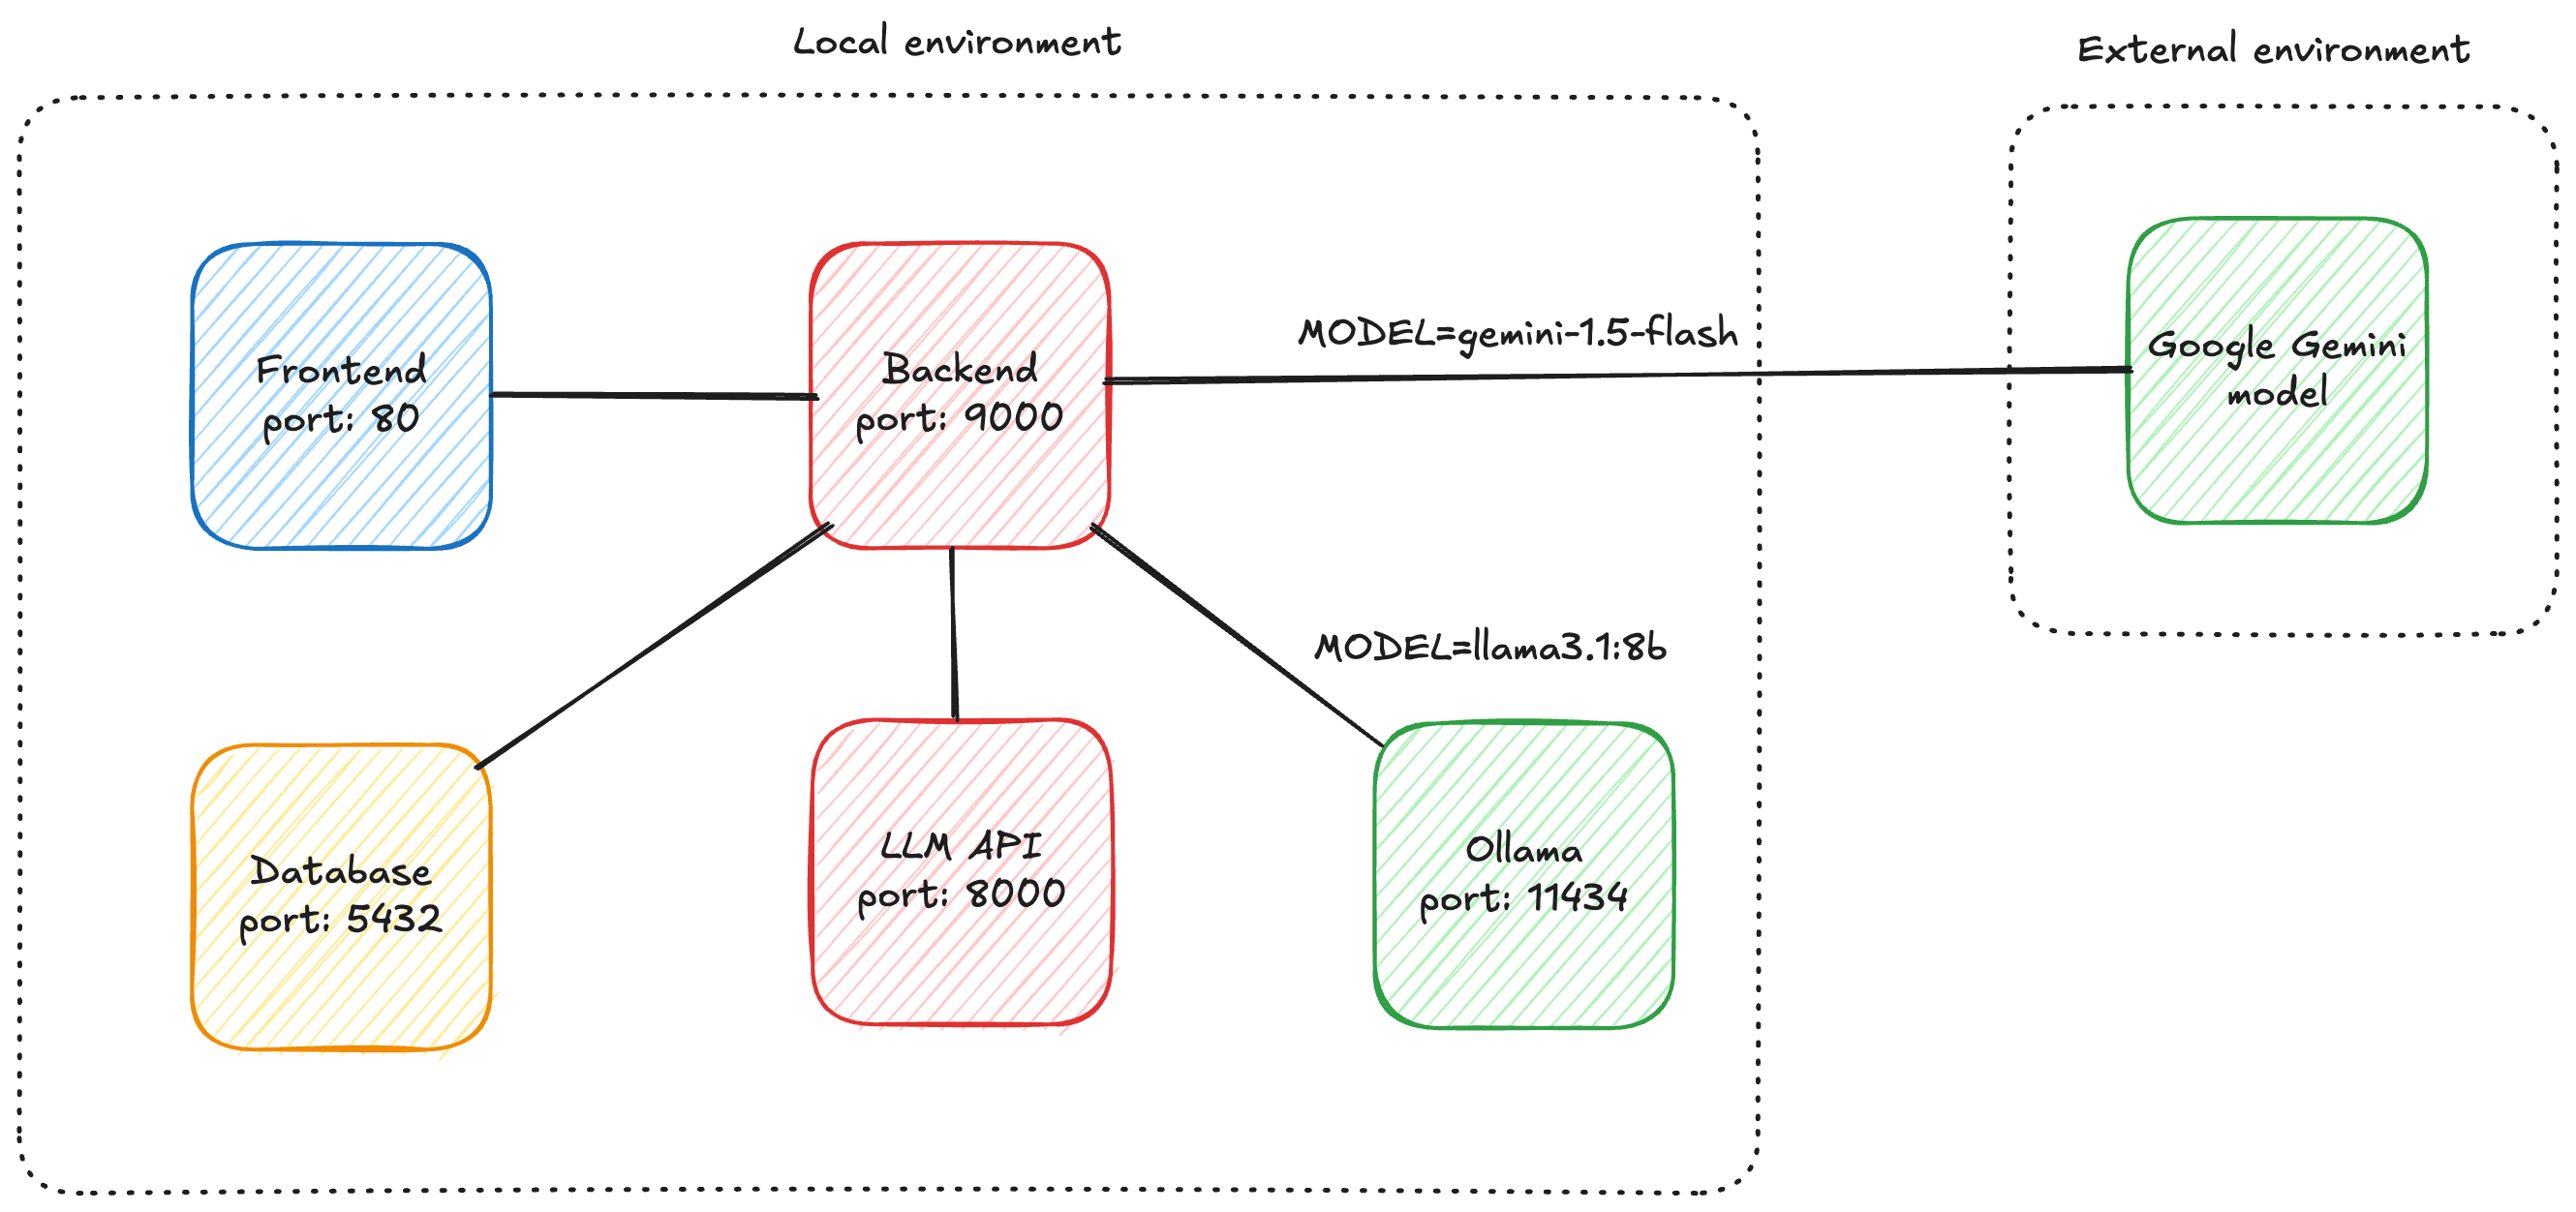
\includegraphics[width=0.8\textwidth, keepaspectratio]{figures/dev-deployment.png}
    \caption{Developer deployment}
    \label{fig:dev-deployment}
\end{figure}

\subsubsection{Production deployment}

We use a similar structure for production but without the Gemini model. We also split up the parts in this case into two, as Figure \ref{fig:production-deployment} shows. The regular services (frontend, backend, database, LLM API) are found on Máté's VPS (Virtual Private Server) in a Kubernetes\footnote{https://kubernetes.io/} cluster, while the AI model is deployed to an external provider. The VPS has no GPU; thus, we selected a provider specializing in running LLMs.

\begin{figure}[!h]
    \centering
    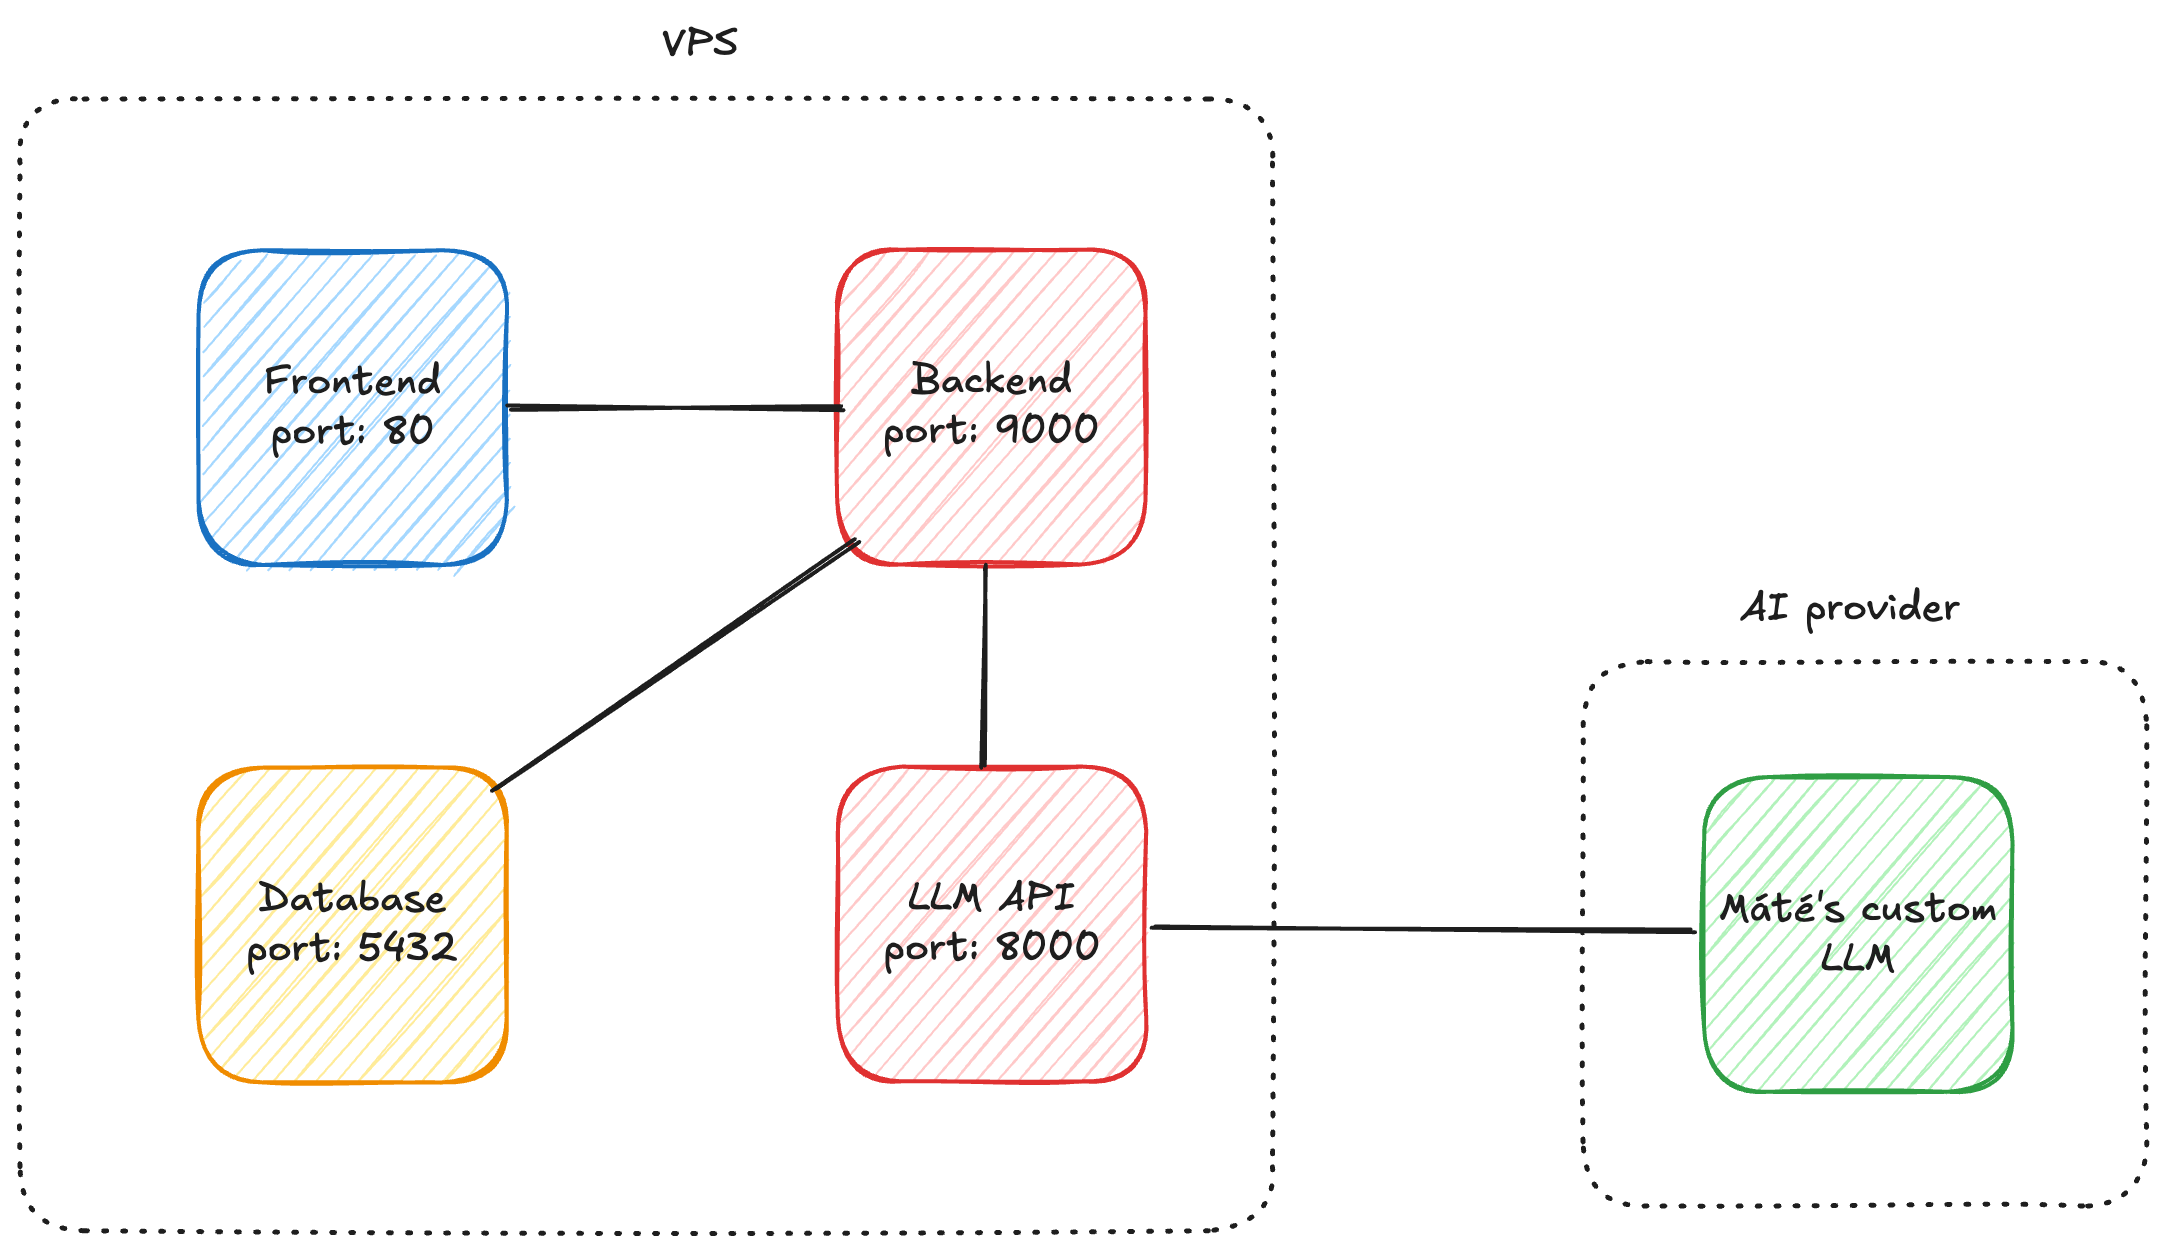
\includegraphics[width=0.8\textwidth, keepaspectratio]{figures/production-deployment.png}
    \caption{Production deployment}
    \label{fig:production-deployment}
\end{figure}

\section{Database Design}

\subsection{Entity-Relationship diagrams}

\subsection{Database schema}

\subsection{Key tables and their relationships}

\subsubsection{Core tables}
    
\subsubsection{Supporting tables}
    
\subsection{Data modeling decisions}

\subsubsection{Indexing strategy}

\subsubsection{Data type selection}

\subsubsection{Constrains and integrity rules}

\section{Frontend Design}

\subsection{User Interface (UI) design principles}

\subsubsection{Chosen design metolodogy}

\subsubsection{User experience (UX) goals}

\subsubsection{Design system planning}

\subsection{Architecture Planning}

\subsubsection{Selected frontend architecture pattern and rationale}
        
I adopted a server-side-driven architecture using HTMX and Go for the application. It is a Multi-Page Architecture (MPA) at the core but leverages the framework's SPA-like capabilities. The architectural pattern consists of server-side HTML generation, HTMX enhancement, and the component structure.

The server generates the pages dynamically using the templating engine called templ. The dynamic content is served through partial HTML updates with HTMX requests. This way, the server controls the UI state instead of the client. The approach has several benefits: it decreases the initial site load and simplifies state management because the client receives the complete page containing the client state.

The HTMX library provides the interactions with its AJAX request boosting feature. Applications using the framework can act like single-page applications because the in-place content updates could replace full-page reloads. The approach offers progressive enhancement by not requiring rewriting everything initially and reduces writing additional JavaScript even to zero lines.

The UI is organized into reusable components. They are written in Go using templ.

\subsubsection{Component hierarchy planning}

\subsubsection{}

\section{Backend Design}

\section{AI integration Design}